\chapter{Апробация в компанию МАГНИТ}\label{vkr_magnit}
% \pdfximage{my_folder/images/vkr_magnit.pdf}%
% \newcount\pdf@totalpages
% \pdf@totalpages=4
% \makeatother

% \newcounter{pdfpage}
% 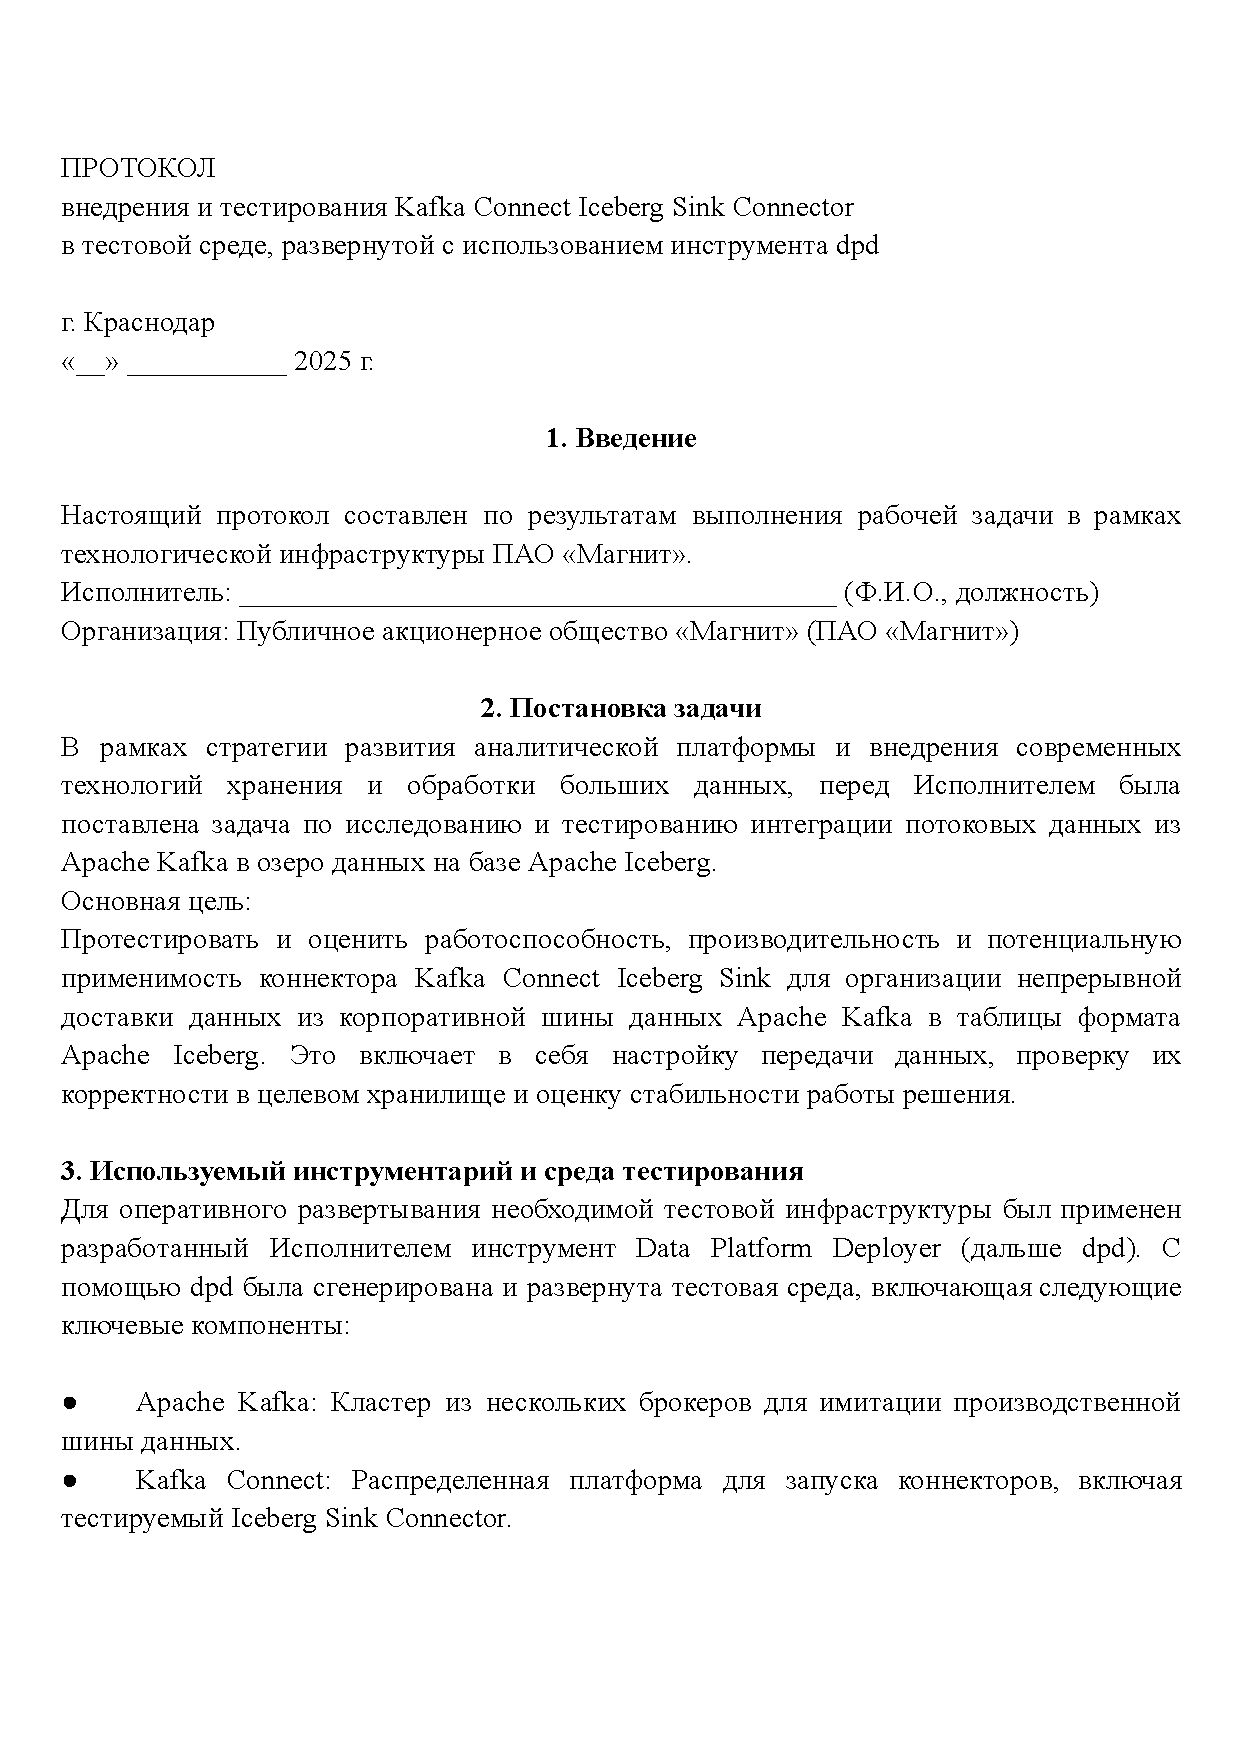
\includepdf[pages=-,scale=0.75]{my_folder/images/vkr_magnit.pdf}
% \begin{figure}
%       \center
%       \includegraphics [%
% pages={1-}, % «–» означает «все страницы»
% width=\textwidth, % подогнать по ширине текстового блока
% height=\textheight, % подогнать по высоте текстового блока
% keepaspectratio % сохранить пропорции, чтобы не было искажен 
%       ]
%       {my_folder/images/vkr_magnit.pdf}
%       \caption{Диаграмма пакетов}
%       \label{fig:vkr_magnit}
% \end{figure}

% \forloop{pdfpage}{1}{\value{pdfpage}<=5}{%

%   % Если нужно, чтобы картинка была по центру:
%   \begin{center}
%     \includegraphics[
%       page=\value{pdfpage},   % номер вставляемой страницы
%       scale=0.75              % ваш коэффициент масштабирования
%       % можно заменить на width=\textwidth, height=\textheight, keepaspectratio
%     ]{my_folder/images/vkr_magnit.pdf}%
%   \end{center}

% тут продолжится ваш текст или следующая картинка
% }

\includegraphics[scale=0.35,page=1]{my_folder/images/act_magnit.PNG}
\clearpage
% \includegraphics[scale=0.75,page=2]{my_folder/images/vkr_magnit.pdf}
% \clearpage
% \includegraphics[scale=0.75,page=3]{my_folder/images/vkr_magnit.pdf}
% \clearpage
% \includegraphics[scale=0.75,page=4]{my_folder/images/vkr_magnit.pdf}
% \clearpage
% \includegraphics[scale=0.75,page=5]{my_folder/images/vkr_magnit.pdf}
% \clearpage
% \includegraphics[scale=0.75,page=6]{my_folder/images/vkr_magnit.pdf}
% \clearpage
% \includegraphics[scale=0.75,page=7]{my_folder/images/vkr_magnit.pdf}
% \clearpage
% \includegraphics[scale=0.75,page=8]{my_folder/images/vkr_magnit.pdf}
% \clearpage

